\documentclass[12pt]{scrbook} %%%http://www.golatex.de/wiki/KOMA-Script%%%

\usepackage{ucs}
\usepackage[utf8x]{inputenc}
\usepackage[ngerman]{babel}
\usepackage{amsmath,amssymb,amstext}
\usepackage{graphicx}


\title{Pferdeführanlage \\ }
\subtitle{HTBLA Kaindorf an der Sulm \\ Grazer Straße 202, A-8430 Kaindorf an der Sulm \\ Ausbildungsschwerpunkt Mechatronik und Automatisierungstechnik}
\author{Ornik Stefan, Riegelnegg Dominik, \\ Freyler Lukas, Pölzl Fabio}
\date{Abgabedatum: \today{}}

\begin{document}

\maketitle
\vfill
\begin{center} 
Betreut von:\\Dipl.-Ing Manfred Steiner\\Dipl.-Ing Wolfgang Mader\\Dipl.-Ing Werner Harnisch\\Dipl.-Päd Otto Schuller
\end{center}
\newpage

\tableofcontents

\listoffigures

\listoftables

%%%%
\newpage
%%%%
\chapter{Einleitung}
\label{sec:einleitung}

\section{Zielsetzung}
\label{sec:zielsetzung}

\subsection{Elektronik}
\label{sec:elektronik}

\section{Gesamtziel}
\label{sec:gesamtziel}
%%%%
\newpage
%%%%
\chapter{Elektronik und Sicherheit}
\label{sec:elektronikUndSicherheit}

\section{Abstract}
\label{sec:abstract}

Because of the electronic part, the horse exerciser should be able to rotate. 
The actuator of the engine is realised by a frequency converter, which gets the signals from the GPIO-Pins on the Raspberry-Pi.
How fast the horse exerciser will move, depends on the commands, that he recives over the Ethernet from the webserver.
The horses will get a refreshment on hot sommer days by the use of the electric water valve.
Due to the fact that the system will be used to exercise animals, one of the most important points is the safety of the horses.

\section{Zusammenfassung}
\label{sec:zusammenfassung}

Der Elektronikteil soll dazu dienen, die Pferdeführanlage in den gewünschten Geschwindigkeiten zu drehen, welche über die App für die Pferde gewählt wurden. 
Die Ansteuerung des Motors kann mit einem Frequenzumrichter realisiert werden, 
welcher die Signale von den GPIO-Pins des Raspberry-Pis bekommt.
Des weiteren bekommt der Raspberry-Pi über Ethernet die Befehle, wie schnell sich die Anlage drehen darf und wie lange. 
Mittels eines elektrischen Wasserventils, wird den Pferden an heißen Sommertagen eine Erfrischung ermöglicht. 
Da mit der Anlage Tiere trainiert werden sollen, ist einer der wichtigsten Punkte die Sicherheit der Pferde.

\section{Aufgabenbereich}
\label{sec:aufgabenbereich}

Mein Aufgabenbereich bei der Diplomarbeit ,,Pferdeführanlage“, ist die Planung für die Elektronik. Wie bereits bei der Hauptaufgabenstellung (1.1.?) erwähnt, 
soll sich die Anlage mit verschiedenen Geschwindigkeiten und Variationen drehen.  Neben der Steuerung der Anlage, muss man auch auf die Sicherheit der Pferde achten.
\\
\\
Mein Aufgabenbereich bei der Diplomarbeit sind:

\begin{itemize}
\item Auswahl des Motors
\item Ansteuerung des Motors
\item Auswahl der Sensoren
\item Auswahl eines Ventils
\item Kommunikation zu Web-Server
\item Schutz des Pferdes
\end{itemize}
%%%%
\newpage
%%%%
\section{Vorarbeit}
\label{sec:vorarbeit}

Um die Suche ein wenig einzugrenzen, wurden persönliche Vorgaben festgelegt.
Diese Vorgaben konnten durch Erfahrung oder Gespräche erstellt werden.

\subsection{Motor}
\label{sec:motor}

Prinzipiell könnte man die Anlage auch rein mechanisch Ansteuern. Mit der Hilfe von Wind, Wasser oder Öl, diese sind aber wetter- und ortsbedingt, im letzten Fall noch eine zusätzliche Umweltbelastung. Da in Mitteleuropa fast jeder Haushalt eine Stromanbindung hat, wurde der Fokus auf die Elektromotoren gerichtet.

\subsection{Ansteuerung Elektromotor}
\label{sec:ansteuerungElektromotor}

Um einen Motor gezielt und einfach steuern zu können, wird in den meisten Fällen auf einen Frequenzumrichter zurückgegriffen. Alternative dazu wäre ein Motorstarter. Mit diesen lassen sich aber nicht so einfach die Geschwindigkeiten steuern.

\subsection{Wasserversorgung Sprühregen}
\label{sec:wasserversorgungSpruehregen}

Für die Wasserversorgung wird ein 1 Zoll Wasseranschluss benötigt. Dieser ist normaler Weise bei jedem Haus vorhanden. 
Sollte dies nicht der Fall sein, ist es auch möglich eine Zuleitung mit geringeren Durchmesser nehmen.

\subsection{Verarbeitung der Daten}
\label{sec:verarbeitungDerDaten}

Da sowohl das Senden von elektrischen Signalen, als auch die Kommunikation über ein Netzwerk realisiert werden soll, wird ein Embedded System verwendet werden.
Dieser ermöglicht sowohl die Funktion eines Computers, als auch technische Funktionen, welche durch zusätzliche Pins am System steuerbar sind.

\subsection{Pferde Sicherheit}
\label{sec:pferdeSicherheit}

Man darf bei der Anlage nicht auf die allgemeine Sicherheit vergessen. Überall können Fehler auftreten. Bei einem Fehler muss man wissen, wie man die Pferde, Menschen und auch die Anlage schützt. Dazu gehören allgemeine Fehler, NOT-AUS und NOT-STOP.
%%%%
\newpage
%%%%

\section{Antriebstechnik Grundlagen}
\label{sec:antriebstechnikGrundlagen}

\subsection{Aufbau}
\label{sec:aufbau}
\begin{figure}[!ht]
\begin{center}
	\caption{Aufbau Antriebstechnik}
	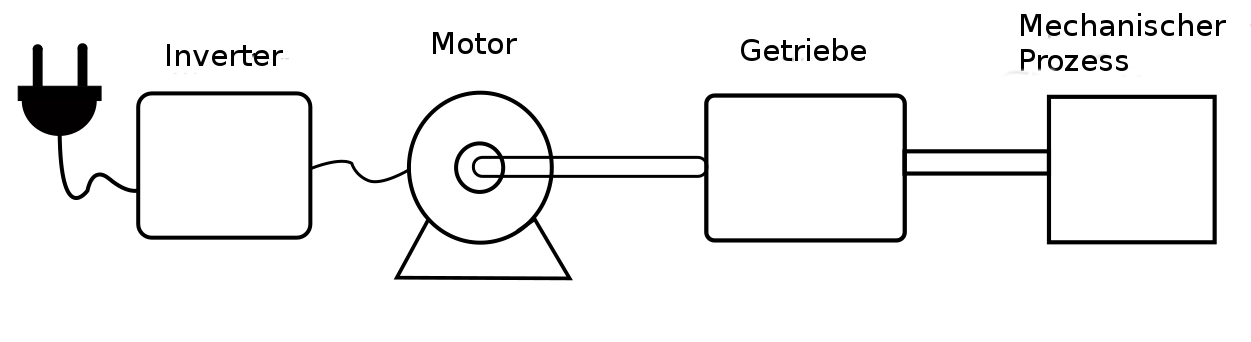
\includegraphics[width=1\textwidth]{AntriebstechnikAufbau}
\end{center}
\end{figure}

Der Inverter wandelt die vorhandene elektrische Energie in die gewünschte elektrische Ausgangsgröße um. 
Diese wird so gewählt, dass der Motor direkt damit betrieben werden kann. Dieser kann mittels der Welle den gewünschten mechanischen Prozess betreiben.  Falls man die Drehzahl nicht elektrisch verändern will, benötigt man zusätzlich ein Getriebe. Das Getribe kann aber auch nur als Verbindung dienen und mittels Keilriemen oder ähnlichem realisiert werden.

Daraus ergibt sich folgender Ablauf wie aus der Abbildung oben ersichtlich:
Versorgungsspannung → Inverter → Motor → (Getriebe) → Mechanischer Prozess

\subsection{Anforderungen}
\label{sec:anforderungen}

Ein Antriebssystem sollte gewissen Anforderungen entsprechen, um vermarktbar zu sein. Folgende Auflistung zeigt die wichtigsten Punkte:

\begin{itemize}
\item{Stabile Steuerung der Geschwindigkeit}
\item{Verbundene Mechanik mit hoher Genauigkeit ansteuern}
\item{Stabile Kraftanwendung}
\end{itemize}

\section{Elektromotor}
\label{sec:elektromotor}

\subsection{Grundprinzip}
\label{sec:grundprinzip}

Die Kraft, welche den Elektromotor in Bewegung versetzt, nennt sich Lorentzkraft.
Befindet sich ein stromdurchflossener elektrischer Leiter in einem Magnetfeld, so wirkt auf diesen Leiter eine Kraft.
Die Wirkungsrichtung hängt von der Stromflussrichtung im Leiter ab. 
Um sich die Vorstellung zu erleichtern, wird in den meisten Fällen die "Linke-Hand-Regel" verwendet.

\begin{figure}[!ht]
\begin{center}
	\caption{Linke-Hand-Regel}
	\includegraphics[width=0.35\textwidth]{LinkehandRegel}
\end{center}
\end{figure}

Die Lorentzkraft wird mit folgender Formel festgelegt:

\begin{equation}
\label{eq:1}
 F = B * I * l
\end{equation}
\begin{center}
F= Lorentzkraft, B= magnetische Flussdichte, \\ I = Stromstärke, l = Länge des Leiters im Magnetfeld
\end{center}

Aus der Formel lässt sich entnehmen, dass die Lorentzkraft von der magnetischen Flussdichte, Stromstärke und Länge des Leiters abhängt.

Diese Kraft erzeugt bei einer Lagerung von der Spule, ein Moment, welches das System drehen lässt

\subsection{Motorarten}
\label{sec:motorarten}

\subsubsection{Gleichstrommotor}
\label{sec:gleichstrommotor}


\subsection{Motorauswahl}
\label{sec:motorauswahl}


\begin{figure}[!ht]
\begin{center}
	\caption{Tabelle Übersicht Elektromotor}
	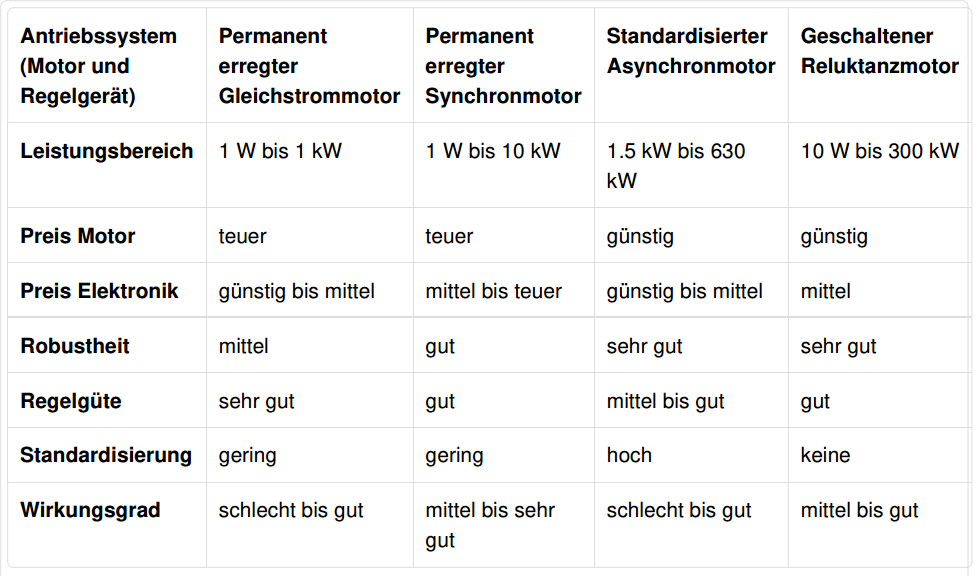
\includegraphics[width=1\textwidth]{TabelleMotor}
\end{center}
\end{figure}

Die Tabelle gibt einen Überblick, in welchen Bereich man seinen gesuchten Motor finden kann. 
Um weiter den gewünschten Motor auswählen zu können, benötigt man die Daten, was überhaupt bewegt werden soll und wie.

\subsubsection{Motoranforderungen}
\label{sec:motoranforderungen}

Der Laufradius der Pferdeführanlage wurde mit 10 Metern angenommen, kann man die Pferde nicht galoppieren lassen. 
Bei Pferden wird ein schneller Trab mit 18 km/h angenommen. %equivetinfo.de/html/eckdaten_pferd.html 5.1.18 16:35%
Um den Motor ein wenig zu entlassen, wird die gewünschte Höchstgeschwindigkeit der Anlage, mit 20km/h angenommen. 
Bei unserem Radius, dreht sich die Konstruktion mit nur 5,3 min\textsuperscript{-1}. 
Durch dem Eigengewicht der Konstruktion kommen auf unserer Pferdeführanlage Trägheitsmomente. 
Die Beschleunigung der Anlage beträgt 0,27m/s². Aufgrund dessen, muss der Motor eine Leistung von ????.W haben und ein Drehmoment von ????.Nm aufbringen können.

Zusammengefasst muss der Motor folgendes Erfüllen:

\begin{itemize}
\item{Drehmoment: ???? Nm}
\item{Leistung: ???? W}
\item{Drehzahl: max. 5,5min\textsuperscript{-1}}
\end{itemize}

\subsubsection{Auswahlverfahren}
\label{sec:auswahlverfahren}

Aufgrund der Anforderungen fiel die Entscheidung auf die Asynchronmotoren. Da die Anlage mit sehr geringer Drehzahl fährt, besteht die Möglichkeit ein externes Getriebe oder direkt auf einen Getriebemotor zurückzugreifen. 
Am Häufigsten findet man bei uns eine 230V Steckdose. Drehstromsteckdosen sind meist nur an den Orten platziert, wo sie von Anfang an benötigt werden. Um den Besitzer keine Umbauarbeiten aufzulegen liegt das Visier bei einen 230V Getriebemotor.

\subsubsection{Getriebemotor}
\label{sec:getriebemotor}

Ein Getriebemotor hat besteht aus einem Motor und einem Getriebe, welche direkt in einer gemeinsamen Einheit miteinander verbunden sind. Das Getriebe soll sowohl Drehzahl als auch Drehmoment des Motors verwandeln. Diese Wandlung kann mittels Drehzahlverhältnis ermittelt werden. Bei Getriebemotoren muss man das Drehmoment von Motor und Getriebe beachten. Primär gilt die Last die auf das Getriebe wirkt. 
Wie auch bei allen anderen Motoren gibt es auch bei den Getriebemotoren viele weitere Modelle. Zum Beispiel Servo-Getriebemotore und Verstellbare-Getriebemotore.

\newpage
%%%%
\subsection{Frequenzumrichter}
\label{sec:frequenzumrichter}
%%%%
\newpage
%%%%
\section{Wasserversorgung}
\label{sec:wasserversorgung}
%%%%
\newpage
%%%%
\section{Geschwindigkeitsmessung}
\label{sec:geschwindigkeitsmessung}
%%%%
\newpage
%%%%
\section{Kommunikationsschnittstelle}
\label{sec:kommunikationsschnittstelle}
%%%%
\newpage
%%%%
\section{Sicherheit der Pferde und Anlage}
\label{sec:sicherheitDerPferdeUndAnlage}

\subsection{Allgemeine Sicherheitsfragen}
\label{sec:allgemeineSicherheitsfragen}

Um die Anlage bei Tieren aktivieren zu können, muss man auch eine Basissicherheit gewährleisten.

Diesen Bereich darf man nicht vernachlässigen. 

In Folgenden Abschnitt  kann nicht auf Besitzer oder Eigentümer Rücksicht genommen werden , da es beide Fälle in der Praxis geben kann.

Bei unserer Pferdeführanlage können folgende Fehler bewusst auftreten:

\begin{itemize}
\item{Was passiert, wenn ein Pferd hinfällt?}
\item{Was passiert wenn ein Pferd stur stehen bleibt?}
\item{Was passiert wenn das Pferd die Anlage anschieben will (schneller ist)?}
\item{Was passiert wenn die Anlage nicht arbeitet wie gewünscht?}
\item{Welche Vorkehrungen gibt es im Bereich Blitzschutz?}
\end{itemize}

\subsection{Tierschutzgesetz und Anlagenschutz}
\label{sec:tierschutzgesetzUndAnlagenschutz}

Gemäß §5 Abs. 1 Tierschutzgesetz ist es verboten, 
einem Tier ungerechtfertigt Schmerzen, Leiden oder Schäden zuzufügen oder es in schwere Angst zu versetzten. 
Unter §5 Abs. 2 Satz 3 lit. b wird nochmals extra darauf hingewiesen, dass keine technischen Geräte verwendet werden, welche das Verhalten eines Tieres durch Härte oder durch Strafreize zu beeinflussen. 

Somit darf man dem Ross mit unserer Anlage, keine kleinen Denkimpulse geben, wenn es stur stehen bleibt. Wenn das Reitvieh stehen bleibt darf ihm und der Anlage selbst nichts passieren. Die einfachste und sicherste Lösung ist, die Anlage zu stoppen. Wenn die Anlage weiter fahren möchte, könnten ungewollte Biegemomente auftreten und somit mechanische Schäden in der Anlage verursachen.

Folgende Vorkehrungen wurden auf der elektrischen Seite zum beidseitigem Schutz getroffen:

Sobald die Auswertung des Sensors merkt, dass die Anlage unfreiwillig stehen bleibt, schaltet die Anlage automatisch ab. Daraufhin muss der jeweilige Eigentümer überprüfen, ob es ein technischer Fehler oder ein Problem beim Pferd vorliegt, bevor er diese wieder in Betrieb nimmt
Die Gitter, hinter beziehungsweise vor dem Pferd, werden zum Schutz des Tieres, nicht elektrisch verbunden.
Welcher Zaun gebaut werden möchte, bleibt dem Eigentümer selbst überlassen.

Sollte man einen Elektrozaun beziehungsweise doch Strom durch die Gitter schicken, werden die Pferde in der Anfangsphase leicht gestresst sein. Sobald sie sich daran gewöhnt haben, funktioniert er wie ein normaler Zaun und die Pferde wissen, dass sie diesen nicht berühren sollten.
Bei den Gittern mit Strom würden die Pferde sogar mehr geschützt werden, wenn sie mit Strom durchflossen werden. Grund dafür ist, dass sich die Pferde an den Stangen Verletzungen zu ziehen könnten, als mit kurzen Stromimpulsen. In Österreich ist dies aber nicht gesetzeskonform.

\subsection{Blitzschutz}
\label{sec:blitzschutz}

Da unsere Pferdeführanlage im Freien steht, darf man auch den Fall eines Blitzeinschlags nicht vernachlässigen. 
Die Durchschnittsanzahl von Blitzen in Österreich sind zirka 5 Blitze pro 1km² in einem Jahr. 
Die Anlage darf nicht in Betrieb genommen werden, wenn der Eigentümer bemerkt, 
dass es in wenigen Minuten ein Gewitter geben könnte.
 Sollte die Anlage während eines Gewitters in Betrieb genommen werden, 
gibt es ein erhöhtes Risiko für die Pferde und der Anlage selbst.
 Die Haftung liegt in diesem Fall bei der Person die die Anlage in dieser Zeit in Betrieb nimmt.

\subsection{Winterschutz}
\label{sec:winterschutz}

Die Zeit wo der Winterschutz unserer Pferdeführanlage in Kraft tritt ist die gleiche wie die Winterreifenpflicht in Österreich. Das heißt vom 1. November bis 15. April die Anlage winterfest gemacht sein. 
\\
\\
In folgenden Bereichen muss ein Winterschutz vorgenommen werden:
\begin{description}
\item[Boden:]
Den Untergrund wo sich die Pferde bewegen muss der Eigentümer selbst wählen. Bei Temperaturen unter 6°C darf der Sprühregen nicht mehr aktiviert werden. Nachdem das Wasser gefroren ist kann das Reitvieh am glatten Boden ausrutschen und gleichzeitig könnte es zu Komplikationen der Pferdeführanlage selbst kommen.

\item[Wasserrohre:]

Um ein langes Leben der Wasserrohre gewährleisten zu können, muss der jeweilige Eigentümer vor den jährlich wiederkommenden Kälteperioden das Wasser aus den Rohren entfernen. Eine der gängigsten Methoden ist es, das Wasser in den Wasserleitungen durch ein kleines Entwässerungsventil zu entleeren. Das elektromagnetische Ventil muss manuel geöffnet werden, damit das Wasser zu rinnen beginnt. Wäre das Ventil geschlossen, könnte das Wasser nicht fließen, da ein Unterdruck in der Leitung erzeugt werden würde. Mittels Druckluft kann auch das restliche Wasser ausgeblasen werden. Somit sind die Wasserrohre für den Winter gerüstet.

\end{description}

\subsection{Redundanz}
\label{sec:redundanz}

Im Bereich Sicherheit von Anlagen kann man häufig den Begriff Redundanz aufschnappen. 

 Redundanz (lat. = Überfluss) ist das Vorhandensein zusätzlicher technischer Komponenten, die für den Betrieb eines Systems oder Gerätes nicht nötig sind, solange keine Störung bzw. kein Ausfall vorliegt. \footnote{http://www.secupedia.info/wiki/Redundanz}

Sollte die Pferdeführanlage vermarktet werden, sollte man die Anlage erweitern. Diese Erweiterung betrifft vor allem die Sicherheit der Pferde.

\begin{center}
	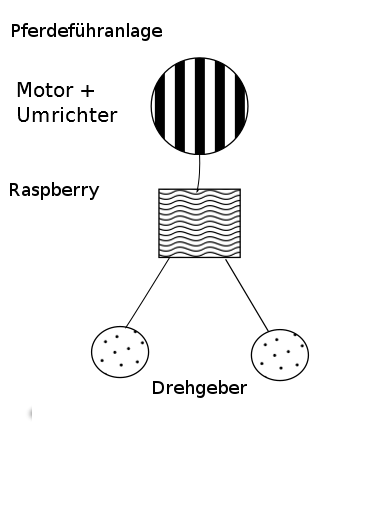
\includegraphics[width=0.5\textwidth]{Redundanz}
\end{center}

Das Bild zeigt eine Möglichkeit die Redundanz zu realisieren.

Gedanke dabei ist, wenn ein Drehgeber defekt ist, kann auch noch der zweite Inkrementalgeber ein Signal liefern, um zumindest einen Durchlaufzyklus beenden zu können. 

\end{document}